%%%%%%%%%%%%%%%%%%%%%%%%%%%%%%%%%%%%%%%%%%%%%%%%%%%%%%%%%%%%%%%%%%%%%%%%
%                                                                      %
%     File: Thesis_Results.tex                                         %
%     Tex Master: Thesis.tex                                           %
%                                                                      %
%     Author: Andre C. Marta                                           %
%     Last modified :  2 Jul 2015                                      %
%                                                                      %
%%%%%%%%%%%%%%%%%%%%%%%%%%%%%%%%%%%%%%%%%%%%%%%%%%%%%%%%%%%%%%%%%%%%%%%%
\chapter{Experimental Evaluation}
\label{chapter:results}

This chapter describes the evaluation of our V2X system, comprised of the PKI Manager and Vehicle Manager. The two main goals of our V2X system are performance and security. With such goals in mind, we designed the evaluation to answer the following questions: 

\begin{enumerate}
	\item Since interoperability is a constant concern, does the system provide acceptable performance? 
	\item Does the system deliver the necessary conditions for vehicle privacy, authentication and overall security?
\end{enumerate}

To perform this evaluation several tests were done regarding the backoffice application, the interaction between the Vehicle Manager and PKI Manager, and the V2X communications within the Vehicle Manager. 

The following sections address these two questions, staring with the performance and resource usage tests, moving to the privacy and security concerns. 

%%%%%%%%%%%%%%%%%%%%%%%%%%%%%%%%%%%%%%%%%%%%%%%%%%%%%%%%%%%%%%%%%%%%%%%%
\section{Performance and Resource Usage}
\label{section:performance}
Performance is a fundamental concern when testing systems that address a sensitive subject such as road safety. The most common metrics of performance are latency and throughput, which correspond to the metrics measured by our tests at different variants. Such tests were performed for the PKI Manager and Vehicle Manager, the environment in which they execute is the following: 

\begin{itemize}
	\item A single installation of the PKI Manager application. 
	\item A basic but functional vehicular PKI including one Root CA, one Enrollment CA, and one Authorization CA.
	\item A single installation of the Vehicle Manager application. 	
\end{itemize}
Ou goal with this setup is to provide a simple but complete V2X environment, where we can use the installation of the PKI Manager to test the performance of the backoffice and RA Service, and use the Vehicle Manager to execute tests focused the resource usage of V2X communications. 

\subsection{PKI Manager}
The PKI Manager is the component of our system which comprises the web application. Therefore, the performance tests done to the PKI Manager have the main goal of understanding how does the application behave under different work load conditions. Such performance tests focus on two aspects: measurements of the latency of the operations supported by the backoffice application, and the communication between client vehicles and the PKI through the RA Service.

Because the PKI Manager tests involve client-server communication over the network, we executed them resorting to two different machines connected throught the same network. The server ran on an Asus laptop with 16GB of RAM and an i7 Intel CPU. For the backoffice testes, the URL was accessed on the browser of the second machine and the measurements were taken using the network tab on the browser's developers console. Regarding the tests to the RA Service, the API of the server, the client vehicles where where generated on the second machine with the usage of \textit{Apache Jmeter} \cite{jmeter}, an open source software designed for testing the performance of web applications. This configuration allows us in both test suits to consider the latency introduced by the network communications aswel as the latency of the processing time at the server. 


\subsubsection{Backoffice Application}
The operations performed by the administrator application are simple but essential in order to have a functional PKI to serve as the backbone of trust within V2X communications. The processing is mostly located at the V2X Library, creating a waiting period on the backoffice application. This is further explained throughout this section which evaluates the latency of the backoffice application.

On the administrator side, it makes sense to only test the latency of the operations performed by one user only, as this application is not meant to be used concurrently by a large number of users. In the remaining part of this section we take a look over the operations evaluated on the backoffice: the generation of keys and certificates. 

In Table \ref{tab:table1} we can observe the time necessary to complete the operations on our backoffice application, disregarding user interaction. The operation to add a key involves the following steps: generating a cryptographic key using the V2X Library, then storing it on a KeyStore and its information on the database. The operation to add a certificate is more complex than the previous, as it also involves searching for the keys which will be relevant to issue the certificate. Because of this factor, we included on the add certificate test the number of keys that exist on the system to provide a comparing factor amongst the different latency times. For each operation the timer started when the form was submitted (POST) and stopped when the page finished loading (GET).

\begin{table}[!htb]
	\renewcommand{\arraystretch}{1.2} % more space between rows
	\centering
	\begin{tabular}{lccc}
		\toprule
		Operation           & $Time$ & $Keys$& $StandardDeviation$ $$\\
		\midrule
		Add key          & 71.6ms & n/a & 14ms   \\
		Add certificate  & 73.7ms &4& 10ms     \\
		Add certificate  & 81ms &20& 13.5ms     \\
		Add certificate  & 128.6ms &40& 16ms     \\
		\bottomrule
	\end{tabular}
	
	\caption[time]{Time needed to add a certificate and a key, calculated over twenty measurements.}
	\label{tab:table1}
\end{table}

The reasoning behind not considering the generation of CAs in the test suit comes from the fact that, unlike the tested operations, generating a CA consists only in creating a simple database object and storing it. 

Overall from the perspective of an administrator the results are reasonable and will not negatively affect the usability of the application. Regarding the operation to add a certificate, the results are what we expected. The more keys that exist on the system at the time of the test, the more time does the system need in order to generate a certificate. This happens due to the nature of the operation, in which the server has to query the database and the KeyStore in order to find the cryptographic keys of the subject and issuer before calling the V2X Library to issue the certificate, and finally storing it on the database. However, the increase in delay is not critical, as considering a realistic number of keys it does not affect the user experience to a point that it is noticeable.

\subsubsection{RA Service}

The RA Service API is the gateway from which the vehicles are able to interact with the PKI to request certificates. Comparing with the backoffice application, the operations done by the RA Service are more complex and subject to more load due to the possibility of concurrent requests from the client vehicles. Therefore, the tests done to this component are designed to evaluate the behaviour of the API at different levels of server load. Ideally, to ensure that the results are as close to the reality as possible, API load tests are run on a production or equivalent system. However, in our case this was not possible so the results may differ depending on the machine which they run. In the remaining part of this section we take a look at the performance tests done to each of the RA Service operations: vehicle configuration, enrollment and authorization.

Table \ref{tab:table2} shows the tests done to the RA Service: latency resulting from the configuration, enrollment and authorization of vehicles respectively. For each operation we performed multiple tests with different numbers of users (threads) requesting that end-point at the same time. We stated with a small number of concurrent requests, then increasing that number in order to increase the load on the server and provide a comparing factor between the latency times. The first column of the table refers to the operation under test. The second shows the number of concurrent threads requesting that operation. Time displays the average latency resulting from ten measurements, where each measurement was taken when the previous was done processing. Throughput gives us an idea of the capacity of the server at the time of those ten measurements, it can be read as the server was processing \textit{x requests / y unit of time}. Finally, the standard deviation enable us to understand the dispersion of the latency times. For each measurement, the timer started when the POST request was submitted by the vehicle, and stopped when the vehicle received the response. That is disregarding the processing done at the client side in order to build the requests and verify the responses. 


 \begin{table}[!htb]
 	\renewcommand{\arraystretch}{1.6} % more space between rows
 	\centering
 	\begin{tabular}{lcccc}
 		\toprule
 		 Operation & $Users$  & $Time$ & $StandardDeviation$ & $ error$$$\\
 		\midrule
 		\multirow{5}{6em}{Configuration}& 1 & 24ms & 3.7ms   \\
 		& 10 & 34ms & 7.7ms     \\
 		& 20& 56ms & 20.2ms     \\
 		& 50& 117 ms& 54ms     \\
 		& 150& 384ms& 183.6ms     \\
 		\hline
 		\multirow{5}{6em}{Enrollment} &1 & 31ms & 13.7ms   \\
 		&10 & 79ms & 33ms     \\
 		&20& 130ms & 62.6ms     \\
 		&50& 276ms & 145ms     \\
 		&150& 856ms & 473.9ms     \\
 		\hline
 		\multirow{5}{6em}{Authorization w/o enrollment validation} &1 & 35ms & 4.5ms   \\
 		&10 & 64ms & 26.1/ms     \\
 		&20& 81ms & 43.3ms     \\
 		&50& 138ms & 68.2ms     \\
 		&150& 325ms & 214.4ms     \\
 			\hline
 		\multirow{5}{6em}{Authorization} &1 & 46ms& 4.4ms   \\
 		&10 & 101ms & 45.5ms     \\
 		&20& 166ms & 90.9ms     \\
 		&50& 346ms & 217.2ms     \\
 		&150& 1567ms & 1069ms & 4.2\%    \\
 		\bottomrule
 		\end{tabular}
 	\caption[time]{Latency measurements for the RA Service operations}
 \label{tab:table2}
\end{table}
 			
\newpage 	
 			
All three operations involve reading the database, and the V2X Library to decode the request and build a response. In addition to this, both the enrollment and authorization of vehicles use the library to validate the vehicle's request and issue the certificate. For the authorization end-point we tested both use cases, as represented by figure \ref{fig:protocol_2}: the authorization process without the enrollment verification, and the full authorization process.

As we can see from the results the authorization of vehicles while verifying their enrollment is the operation which overall introduces more latency. This happens due to the fact this operation is the most complex in terms of computation. Specifically, in the request validation where this version of the vehicle authorization requires the validation of two signatures: the signature that proves the possession of the verification keypair, and the vehicle's enrollment signature. In addition to this, the vehicle's enrollment credential is also verified.

The second operation which introduces more latency for the same number of users is the enrollment of vehicles. Comparing to the previous operation the enrollment of vehicles is simpler. The main difference comes from the validation of the vehicle's request, which in this case only requires the validation of two signatures: the canonical signature and the proof of possession signature. However, as we can see from the results the enrollment introduces almost as much latency as the most complex operation. This is because, Unlike the previous operation, the enrollment of vehicles also requires saving on the database each enrollment credential issued, which introduces a latency bottleneck on the enrollment operation and levels the waiting period with the more complex authorization.

Perhaps the most interesting comparison allowed by these tests is the comparison of the latency introduced by the two different vehicle authorization methods. As we can see from the results, the authorization without vehicle configuration introduced by our RA Service is on average faster than the standard full authorization flow. Since this version of the authorization is the most common use case, the performance gains mean that the efforts presented in Section \ref{protocol} to optimize the authorization process as a whole were succesful from a performance point of view. 

As expected the configuration of vehicles, being the simpler operation, introduced the least latency. Unlike the previous operations, the configuration of vehicles does not require signature validation at the application level or issuing certificates. It mainly requires decoding the request from the vehicle and read/writes to the database. However, the configuration of vehicles shares the same problem as the enrollment operation, as the number of concurrent requests increases, the inserts on the database become more and more expensive. At a hundred and fifty user mark it becomes almost as slow as the authorization of vehicles w/o enrollment validation which is an operation that in terms of business logic is more complex. 

One way to solve the problem shared by the configuration and enrollment operations is to increase the scalability of the data access layer by effectively managing the database writes. This can be achieved by using batch calls instead of single insert calls. Since we are using the default single insert calls, the number of writes results in same number of SQL \textit{insert} operations, which in turn result in that equal number of database round rips. Batching is a mechanism capable of grouping the \textit{inserts}, reducing the database round trips, and consequently increasing the performance of the data access layer. 

A recurrent event that started to happen at the hundred and fifty user mark for all operations was that sometimes unexpected errors started to appear causing the response from the server to be marked a as failed. A possible solution would be to introduce parallelism into the network and distributing the computation. A load balancer would be used distribute the work load between several back-end servers, increasing the number of requests needed to reach a peak in work load and increasing the system's scalability. 



\subsection{Vehicle Manager}
\label{section:memory}
At the Vehicle Manager level, the focus of the performed tests shits from performance to resource usage. This is because the performance of the V2X communications could not be accurately measured by only using the Vehicle Manager. In the previous cases where the performance of the web application was tested we were able to relate the number of users to the latency needed to complete certain operations, which gave a general idea of how the system reacts under different work loads. This is not the case with the Vehicle Manager. The time needed to send messages from one vehicle to another, which are represented by objects within the Vehicle Manager, depends entirely on the system which the application is running. Without access to vehicle specialized V2X hardware the time which the test computer took in order to generate, send and validate V2X messages it not conclusive. In addition to this, the network latency resulting from sending messages could not be accurately simulated because the communications within the Vehicle Manager's vehicles are represented by simple method calls. 

As described in Section \ref{etsi_design} all vehicles have to store different certificates on their local system. In order to have a general notion of the possible quantities and the necessary storage capacity, table \ref{tab:table3} lists the type of certificates, their size, and possible quantity. To estimate the size of the different certificates we used the \textit{java.lang.instrumentation} package \cite{instrumentation}, where we measured size of the ASN.1 COER encoded certificates (i.e. encoded using the V2X Library methods). Regarding the possible quantiy of ATs stored within the vehicles, the values are estimated considering the AT usage pattern presented in Section \ref{section:at_usage}, were we assumed a vehicle using on average five certificates per day with a refill time of a one year. As we can see from the estimation, the authorization tickets and their corresponding private keys are the elements which demand more storage space, corresponding to approximately 87\% of total. It is also important to note that the number of the certificates can change from vehicle to vehicle depending on the usage pattern and the desired level of privacy. This is further discussed in the following section.

\begin{table}[!htb]
	\renewcommand{\arraystretch}{1.2} % more space between rows
	\centering
	\begin{tabular}{lccc}
		\toprule
		Certificate & $Size$ & $Quantity$& $TotalSize$ \\
		\midrule
		Root CA         & 272 bytes & 20 &5.4KB \\
		Enrollment CA  & 288 bytes &100&28.8KB \\
		Authorization CA  & 288 bytes&100&28.8KB\\
		Enrollment Credential  & 208 bytes &1 & 0.2 KB\\
		Authorization Ticket  & 200 bytes &1825 & 365KB\\
		AT private key & 32 bytes & 1825 & 58.4KB\\
		\midrule
		\null  & \null & \null & 486.6KB\\
		\bottomrule
		\end{tabular}
		
		\caption[time]{Estimated vehicle certificate storage demand}
		\label{tab:table3}
	\end{table} 


\section{Security and privacy}
\label{section:pricacy}
When considering security measures to protect a system and its users, the best aproach is to look at meathods which are already implemented and established by trusted entities. 
Our system follows this guideline, we did not implement the security tools from scratch, instead we reused existing implementation were the security is assured by the already existing libraries.
In this section we analyse the security properties considered by our system and study how the privacy of the vehicles is maitained within the PKI and V2X communications.

\subsection{Confidentiality}
Confidentiality over the communications in an important characteristic of our system. Because it is not in the scope of V2X communications to restrict access to messages to certain users, the confidentiality aspect of our system only applies to the communication between the Vehicle Manager and PKI Manager.

To ensure confidentiality, all the information transmitted from and to the client is sent through an SSL secure channel. In this communication channel the Vehicle Manager is authenticated, where the server requires its certificate in order to accept communications. 

In addition, we also provide application level encryption where every certificate request is encrypted by the vehicle so that only the intended recipient CA is able to decrypt it. This feature combined with the encryption of the response to the original vehicle allows the confidentiality of the vehicle's identity, preventing its disclosure during the certificate requests.
 
\subsection{Data Authenticity}
In a system that deals with transmission of messages, confidentiality alone is not enough to assure a secure communication. Data authenticity enables the receptor of a message to confirm the origin and integrity of the data. In our system, this concept applies to both the client-server communication and V2X messages.

Regarding the Vehicle to PKI communication, the authenticity of the messages is achieved at two levels: first at the channel and then application. When the vehicles are generated, the RA trusts the new connections because of the SSL connection with the Vehicle Manager, which can be seen as the vehicle manufacturer. However, after the configuration of such vehicles the authenticity of their certificate requests is achieved at the application level, through the use of digital signatures.

The authenticity of the V2X messages is a similar process where the recipient of a message is able to trust the authenticity of the message by verifying the signature of the sender against a trusted certificate chain. 

\subsection{Authorization}
Authorization over services requires user authentication. In our system this is applied in two aspects: the authentication of the administrator to manage the PKI and the client vehicles to request certificates. 

The authentication of the administrator is accomplished through the use of a username/password mechanism, where the credentials are stored within the database of the server. Specifically, the password is hashed with the \textit{Bcrypt} algorithm before being saved to avoid mainlining it in clear text. The implementation of the hashing function is provided by \textit{Spring Security} and is prepared to internally generate and maintain a random salt value to be hashed alongside the password.

Regarding the authorization of the vehicles, this is achieved through the RA service of vehicle configuration. Only vehicles which completed this service are recognized by our server and are able to request certificates.
  
\subsection{Database breaches}
The access to the data stored within the database is protected by username/password authentication. In addition to this, the access privileges are different depending on the type of user accessing it.

\subsection{Privacy}
In our system the privacy of the users is one of the most important security concerns. Losing privacy might mean that the tracking of vehicles is aided by the V2X communications, which is undesired. The main system variables that might affect the privacy of its users are the number of pseudonym certificates, and the usage pattern. As we know, the more pseudonym certificates a vehicle has available, the better is the privacy. However, as described in the previous sections the increase of privacy comes with the overhead of the increase in certificate storage demand, number of individual certificate requests, and consequently processing at the vehicle side. In this section we analize different V2X scenarios, where we relate a vehicle's movement pattern, the pseudonym usage, possible types of attackers and the resulting level of privacy.

Regarding the types of vehicle trips, we wanted to choose real life cases where V2X communications could be involved. For the privacy scenarios we considered the following cases:
\begin{itemize}
	\item \textbf{Case A:} Round trip, the typical daily home to work commute.
	\item \textbf{Case B:} Trip to a location, from point A to B.
\end{itemize}


The usage of certificates to sign V2X messages introduces privacy concerns over the communication. Therefore, the pattern which vehicles use pseudonyms and the frequency in which the certificate are changed are very impactful variable. We considered the following pattens:
\begin{itemize}
	\item \textbf{Pattern A:} The vehicle always uses different pseudonyms.
	\item \textbf{Pattern B:} For a period of time the vehicle uses all the available pseudonyms then, if necessary, reuses the certificates in a different order.
\end{itemize}

To represent a challenge to the system's privacy, we choose different types of attackers differentiated by their power to capture messages within an area of operation.
\begin{itemize}
	\item \textbf{Attacker A:} Controls a single section on the road while being able to visualize the victim vehicle and capture all messages.
	\item \textbf{Attacker B:} Controls two distant sections on the road where the victim vehicle will pass.  
	\item \textbf{Attacker C:} Attacker is moving for a limited period of time following the victim vehicle. 
\end{itemize}
	
Starting with the least privacy, vehicles with usual round trips using the certificate usage pattern B and low certificate change frequency (e.g. using the same certificate for hours) are vulnerable to all types of attackers. In the case of the attacker A there is a window of vulnerability if the vehicle passes the area controlled by the attacker twice with the same pseudonym. In this case the attacker is able to map that pseudonym to the victim's vehicle. Eventually, when the vehicle reuses the compromised pseudonym it may be possible for the attacker, if capturing the messages, to infer the vehicle's route. The same situation happens when considering the attacker B but with a bigger window of opportunity as the vehicle passes the areas controlled by the attacker twice as more. Because the frequency of certificate change is low it directly affects the privacy of the vehicle when considering the attacker C. In this case, the more time the vehicle uses the same certificate the bigger the probability of the attacker seeing that constant message broadcast by the vehicle, therefore mapping the used pseudonym to the identity of the vehicle and enabling short-term tracking. Despite the fact that this pseudonym usage pattern is worst in terms of privacy for the vehicles usually commuting, it is the least expensive in terms of certificate storage demand because the vehicle is reusing certificates with a low change frequency. 

A privacy improvement for the same conditions would be to increase the frequency in which the vehicle changes pseudonyms. In this case, the vehicle would be more protected against the three types of attackers. In the case of attacker A and B, this is achieved because it would reduce the risk of the vehicle still be using the same certificate while passing through the zone(s) controlled by the attacker. The increase in privacy against attacker C is based on the unlinkability attribute of the pseudonym certificates. This means that when a vehicle changes pseudonym the new certificate can not be mapped to the old, therefore reducing the ability of the attacker to infer which certificate belongs to the vehicle. However, in order to assure the unlinkability of the pseudonym certificates care must be taken regarding the aggregation of information written on the certificate. For example, if a set of the vehicle's certificates have the exact same expiration date an attacker could infer that they belong to the same vehicle, disrupting the unlikability of the affected certificates. 

The best privacy for this type of vehicle movement is achieved through the usage the certificate pattern B. Because certificates are not reused, even if the attacker manages to map a pseudonym to the victim's vehicle it is only possible to track the vehicle for the duration that it uses that certificate (short-term tracking). Increasing the certificate change frequency will further reduce the power of the attacker. 


Considering the vehicle trip B where the vehicle does not pass the same road twice, the privacy is affected practically the same way as in the previous scenarios with trip A. The only difference is when considering the reusage of certificates and attackers of type A and B. In this case, the power of the attacker is reduced because the vehicle will pass each controlled area just one. Therefore, reducing the chance of the attacker to map the pseudonym to the vehicle and compromising the certificate for the reuse. 

A general rule of thumb that is important to consider when using pseudonyms is that a pseudonym is only effective in a crowd. In or case this means that a pseudonym certificate is only effective if there are more vehicles around using them. If a vehicle is isolated on a road sending V2X messages signed with a pseudonym certificate then that certificate can be immediately mapped to the sender, even considering a high pseudonym change frequency.

We have seen in the scenarios that reusing pseudonyms is particularly vulnerable to attacks where the attacker is able to map a specific certificate to a vehicle. The more certificates compromised the bigger the chance of the attacker to infer a vehicle's route by observing the compromised certificates being reused at different locations. However, assuming that vehicles carry thousands of pseudonyms, a few compromised certificates might not be conclusive for the attacker. It all depends on the power of the attacker to compromise certificates by controlling areas and/or following the victim vehicle, the number of certificates reused by the vehicle, and the randomness in which they are selected. We also have seen that having a low pseudonym change frequency is particularly vulnerable to short-term tracking attacks where the attacker is following the vehicle and is able to: see the vehicle using the certificate while isolated, or infer it by the captured messages which are signed constantly by the same certificate. We concluded that the best way to grant privacy is to increase the number of pseudonyms, which enables the possibility of a higher pseudonym change frequency and lowers the need to reuse certificates. But more concretely what is the price in terms of storage in order to have acceptable privacy? 

It depends on the travel distance of the vehicles. In the previous section, we estimated that if a vehicle uses on average 5 pseudonyms in a day with a refill time of one year it would need approximately 486.6KB of certificate storage space. Depending on the distance that a vehicle travels each day, it may need to use more that 5 certificates resulting in the reusage of certificates, and privacy loss in the most cases. To assure that this does not happen a vehicle that spends more time on the road needs more certificates. For example, assuming a vehicle changes certificate each 10 minutes and an average travel time of 2 hours each day. The vehicle would need approximately 12 certificates a day in a total of 4380 for a year. Assuming the same number of PKI certificates as in the previous section \ref{section:memory}, this number of pseudonyms would increase the storage demand to approximately 1MB.

    
\subsection{Summary}
In the end the results from the performed tests are as expected. Regarding the security, we feel that the used technologies and protocols are satisfactory and sufficient. However, the security of the vehicle configuration, which represents the first interaction between the Vehicle Manager and PKI Manager, could be further improved as of now it only depends on the SSL protocol. The privacy of V2X communications as an integral part of the system's security cannot be optimized by choosing a fixed strategy, care must be taken in order to understand the vehicle's routines and finding a compromise between the privacy its associated overheads.

While not the main focus of this system, the performance of the API is also something to take into consideration. Overall we think that the results are acceptable considering the complexity of the operations. However, when increasing the work load on the server by increasing the number of concurrent users, the operations started to take considerable more time to be performed and in some cases errors where introduced. While this is problem for this particular proof of concept system, it can be easily corrected by introducing a distributed infrastructure with several machines to share the work load. In a real life scenario the scalability of the system assumes a much more impactful role considering the sheer number of existing vehicles, and the number of certificate requests done by each vehicle in order to participate in V2X communications. We feel that our contribution with the introduction of the RA Service is able to improve the interaction of the vehicles with the PKI in order to request such certificates and also increase the performance of the vehicle's authorization process by aggregating the requests and only validation the enrolment on the first authorization.





%%%%%%%%%%%%%%%%%%%%%%%%%%%%%%%%%%%%%%%%%%%%%%%%%%%%%%%%%%%%%%%%%%%%%%%%
\begin{comment}

\section{Baseline Solution}
\label{section:baseline}

Analysis of the baseline solution...


%%%%%%%%%%%%%%%%%%%%%%%%%%%%%%%%%%%%%%%%%%%%%%%%%%%%%%%%%%%%%%%%%%%%%%%%
\section{Enhanced Solution}
\label{section:enhanced}

Quest for the optimal solution...


% ----------------------------------------------------------------------
\subsection{Figures}
\label{subsection:figures}

Insert your section material and possibly a few figures...

Make sure all figures presented are referenced in the text!


% ----------------------------------------------------------------------
\subsubsection{Images}
\label{subsection:images}

\begin{figure}[!htb]
  \centering
  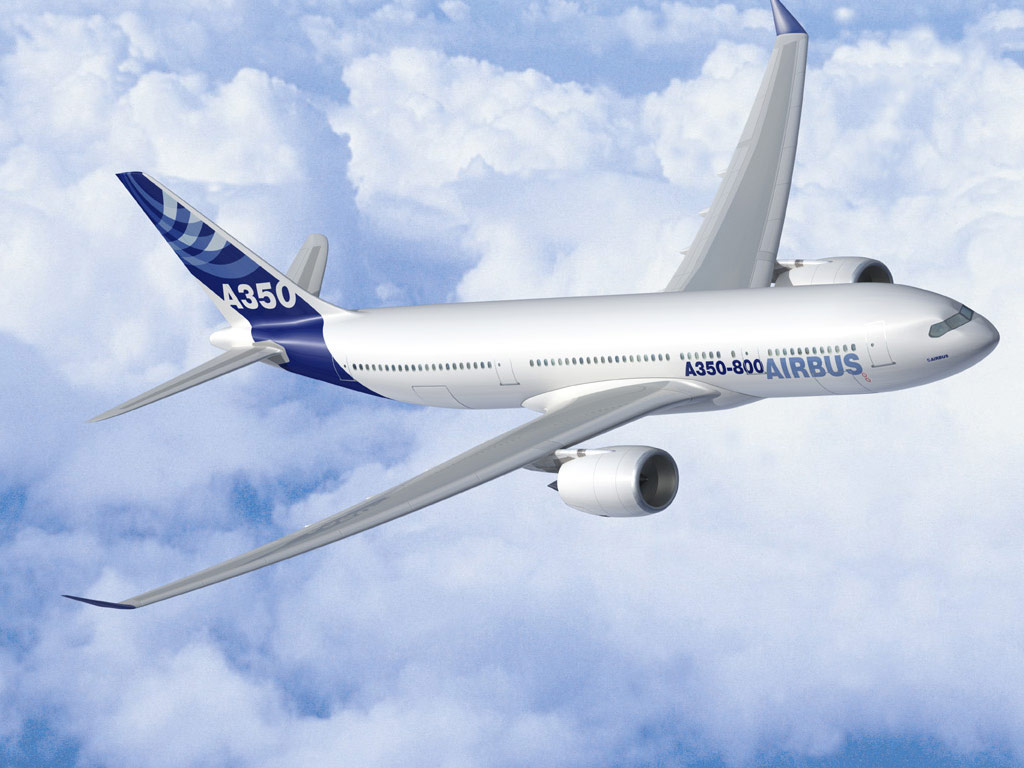
\includegraphics[width=0.25\textwidth]{Figures/Airbus_A350.jpg}
  \caption[Caption for figure in TOC.]{Caption for figure.}
  \label{fig:airbus1}
\end{figure}

\begin{figure}[!htb]
  \begin{subfigmatrix}{2}
    \subfigure[Airbus A320]{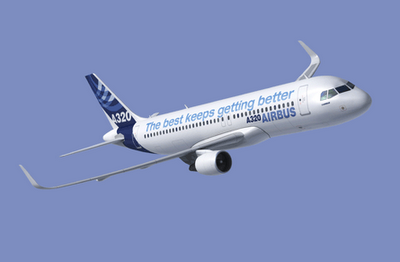
\includegraphics[width=0.49\linewidth]{Figures/Airbus_A320_sharklets.png}}
    \subfigure[Bombardier CRJ200]{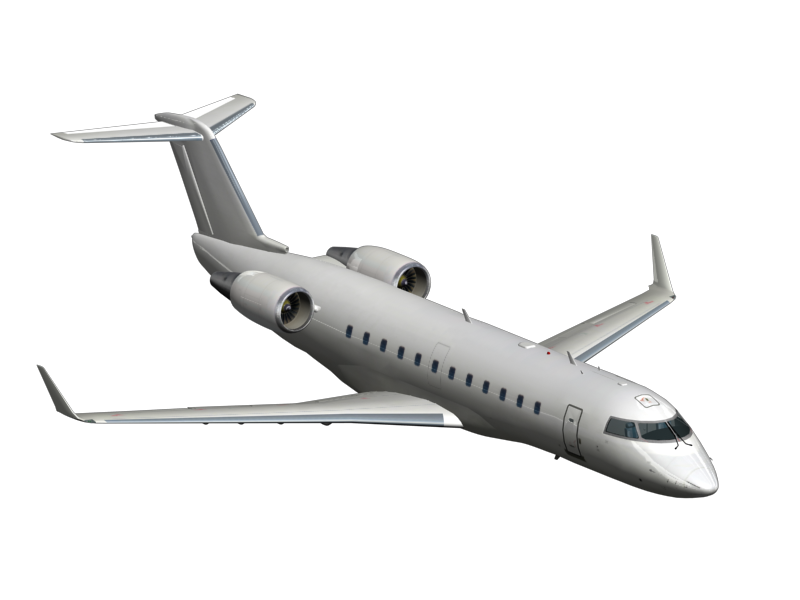
\includegraphics[width=0.49\linewidth]{Figures/Bombardier_CRJ200.png}}
  \end{subfigmatrix}
  \caption{Some aircrafts.}
  \label{fig:aircrafts}
\end{figure}

Make reference to Figures \ref{fig:airbus1} and \ref{fig:aircrafts}.

By default, the supported file types are {\it .png,.pdf,.jpg,.mps,.jpeg,.PNG,.PDF,.JPG,.JPEG}.

See \url{http://mactex-wiki.tug.org/wiki/index.php/Graphics_inclusion} for adding support to other extensions.


% ----------------------------------------------------------------------
\subsubsection{Drawings}
\label{subsection:drawings}

Insert your subsection material and for instance a few drawings...

The schematic illustrated in Fig.~\ref{fig:algorithm} can represent some sort of algorithm.

\begin{figure}[!htb]
  \centering
  \scriptsize
%  \footnotesize 
%  \small
  \setlength{\unitlength}{0.9cm}
  \begin{picture}(8.5,6)
    \linethickness{0.3mm}

    \put(3,6){\vector(0,-1){1}}
    \put(3.5,5.4){$\bf \alpha$}
    \put(3,4.5){\oval(6,1){}}
    %\put(0,4){\framebox(6,1){}}
    \put(0.3,4.4){Grid Generation: \quad ${\bf x} = {\bf x}\left({\bf \alpha}\right)$}

    \put(3,4){\vector(0,-1){1}}
    \put(3.5,3.4){$\bf x$}
    \put(3,2.5){\oval(6,1){}}
    %\put(0,2){\framebox(6,1){}}
    \put(0.3,2.4){Flow Solver: \quad ${\cal R}\left({\bf x},{\bf q}\left({\bf x}\right)\right) = 0$}

    \put(6.0,2.5){\vector(1,0){1}}
    \put(6.4,3){$Y_1$}

    \put(3,2){\vector(0,-1){1}}
    \put(3.5,1.4){$\bf q$}
    \put(3,0.5){\oval(6,1){}}
    %\put(0,0){\framebox(6,1){}}
    \put(0.3,0.4){Structural Solver: \quad ${\cal M}\left({\bf x},{\bf q}\left({\bf x}\right)\right) = 0$}

    \put(6.0,0.5){\vector(1,0){1}}
    \put(6.4,1){$Y_2$}

    %\put(7.8,2.5){\oval(1.6,5){}}
    \put(7.0,0){\framebox(1.6,5){}}
    \put(7.1,2.5){Optimizer}
    \put(7.8,5){\line(0,1){1}}
    \put(7.8,6){\line(-1,0){4.8}}
  \end{picture}
  \caption{Schematic of some algorithm.}
  \label{fig:algorithm}
\end{figure}


% ----------------------------------------------------------------------
\subsection{Equations}
\label{subsection:equations}

Equations can be inserted in different ways.

The simplest way is in a separate line like this

\begin{equation}
  \frac{{\rm d} q_{ijk}}{{\rm d} t} + {\cal R}_{ijk}({\bf q}) = 0 \,.
\label{eq:ode}
\end{equation}

If the equation is to be embedded in the text. One can do it like this ${\partial {\cal R}}/{\partial {\bf q}}=0$.

It may also be split in different lines like this

\begin{eqnarray}
  {\rm Minimize}   && Y({\bf \alpha},{\bf q}({\bf \alpha}))            \nonumber           \\
  {\rm w.r.t.}     && {\bf \alpha} \,,                                 \label{eq:minimize} \\
  {\rm subject~to} && {\cal R}({\bf \alpha},{\bf q}({\bf \alpha})) = 0 \nonumber           \\
                   &&       C ({\bf \alpha},{\bf q}({\bf \alpha})) = 0 \,. \nonumber
\end{eqnarray}

It is also possible to use subequations. Equations~\ref{eq:continuity}, \ref{eq:momentum} and \ref{eq:energy} form the Naver--Stokes equations~\ref{eq:NavierStokes}.

\begin{subequations}
    \begin{equation}
    \frac{\partial \rho}{\partial t} + \frac{\partial}{\partial x_j}\left( \rho u_j \right) = 0 \,,
    \label{eq:continuity}
    \end{equation}
    \begin{equation}
    \frac{\partial}{\partial t}\left( \rho u_i \right) + \frac{\partial}{\partial x_j} \left( \rho u_i u_j + p \delta_{ij} - \tau_{ji} \right) = 0, \quad i=1,2,3 \,,
    \label{eq:momentum}
    \end{equation}
    \begin{equation}
        \frac{\partial}{\partial t}\left( \rho E \right) + \frac{\partial}{\partial x_j} \left( \rho E u_j + p u_j - u_i \tau_{ij} + q_j \right) = 0 \,.
    \label{eq:energy}
    \end{equation}
\label{eq:NavierStokes}%
\end{subequations}


% ----------------------------------------------------------------------
\subsection{Tables}
\label{section:tables}

Insert your subsection material and for instance a few tables...

Make sure all tables presented are referenced in the text!

Follow some guidelines when making tables:

\begin{itemize}
  \item Avoid vertical lines
  \item Avoid “boxing up” cells, usually 3 horizontal lines are enough: above, below, and after heading
  \item Avoid double horizontal lines
  \item Add enough space between rows
\end{itemize}

\begin{table}[!htb]
  \renewcommand{\arraystretch}{1.2} % more space between rows
  \centering
  \begin{tabular}{lccc}
    \toprule
    Model           & $C_L$ & $C_D$ & $C_{M y}$ \\
    \midrule
    Euler           & 0.083 & 0.021 & -0.110    \\
    Navier--Stokes  & 0.078 & 0.023 & -0.101    \\
    \bottomrule
  \end{tabular}
  \caption[Table caption shown in TOC.]{Table caption.}
  \label{tab:aeroCoeff}
\end{table}

Make reference to Table \ref{tab:aeroCoeff}.

Tables \ref{tab:memory} and \ref{tab:multipleColumns} are examples of tables with merging columns:

\begin{table}[!htb]
  \renewcommand{\arraystretch}{1.2} % more space between rows
  \centering
  \begin{tabular}[]{lrr}
    \toprule
                & \multicolumn{2}{c}{\underline{Virtual memory [MB]}} \\
                & Euler       & Navier--Stokes \\
    \midrule
      Wing only &  1,000      &    2,000       \\
      Aircraft  &  5,000      &   10,000       \\
      (ratio)   & $5.0\times$ & $5.0\times$    \\
    \bottomrule
  \end{tabular}
  \caption{Memory usage comparison (in MB).}
  \label{tab:memory}
\end{table}

\begin{table}[!htb]
  \centering
  \renewcommand{\arraystretch}{1.2} % more space between rows
  \begin{tabular}{@{}rrrrcrrr@{}} % remove space to the vertical edges @{}...@{}
    \toprule
      & \multicolumn{3}{c}{$w = 2$} & \phantom{abc} & \multicolumn{3}{c}{$w = 4$} \\
    \cmidrule{2-4}
    \cmidrule{6-8}
      & $t=0$ & $t=1$ & $t=2$ && $t=0$ & $t=1$ & $t=2$ \\
    \midrule
      $dir=1$
      \\
      $c$ &  0.07 &  0.16 &  0.29 &&  0.36 &  0.71 &   3.18 \\
      $c$ & -0.86 & 50.04 &  5.93 && -9.07 & 29.09 &  46.21 \\
      $c$ & 14.27 &-50.96 &-14.27 && 12.22 &-63.54 &-381.09 \\
      $dir=0$
      \\
      $c$ &  0.03 &  1.24 &  0.21 &&  0.35 & -0.27 &  2.14 \\
      $c$ &-17.90 &-37.11 &  8.85 &&-30.73 & -9.59 & -3.00 \\
      $c$ &105.55 & 23.11 &-94.73 &&100.24 & 41.27 &-25.73 \\
    \bottomrule
  \end{tabular}
  \caption{Another table caption.}
  \label{tab:multipleColumns}
\end{table}

An example with merging rows can be seen in Tab.\ref{tab:multipleRows}.

\begin{table}[!htb]
  \renewcommand{\arraystretch}{1.2} % more space between rows
  \centering
  \begin{tabular}{ccccc}
    \toprule
      \multirow{2}{*}{ABC} & \multicolumn{4}{c}{header} \\
      \cmidrule{2-5} & 1.1 & 2.2 & 3.3 & 4.4 \\
    \midrule
      \multirow{2}{*}{IJK} & \multicolumn{2}{c}{\multirow{2}{*}{group}} & 0.5 & 0.6 \\
      \cmidrule{4-5}       & \multicolumn{2}{c}{}                       & 0.7 & 1.2 \\
    \bottomrule
  \end{tabular}
  \caption{Yet another table caption.}
  \label{tab:multipleRows}
\end{table}

If the table has too many columns, it can be scaled to fit the text widht, as in Tab.\ref{tab:scale}.
\begin{table}[!htb]
  \renewcommand{\arraystretch}{1.2} % more space between rows
  \centering
  \resizebox*{\textwidth}{!}{%
    \begin{tabular}[]{lcccccccccc}
      \toprule
        Variable &  a  &  b  &  c  &  d  &  e  &  f  &  g  &  h  &  i  &  j  \\
      \midrule
        Test 1   &  10,000 &  20,000 &  30,000 &  40,000 &  50,000 &  60,000 &  70,000 &  80,000 &  90,000 & 100,000 \\
        Test 2   &  20,000 &  40,000 &  60,000 &  80,000 & 100,000 & 120,000 & 140,000 & 160,000 & 180,000 & 200,000 \\
      \bottomrule
    \end{tabular}
  }%
  \caption{Very wide table.}
  \label{tab:scale}%
\end{table}


% ----------------------------------------------------------------------
\subsection{Mixing}
\label{section:mixing}

If necessary, a figure and a table can be put side-by-side as in Fig.\ref{fig:side_by_side}

\begin{figure}[!htb]
  \begin{minipage}[b]{0.60\linewidth}
    \centering
    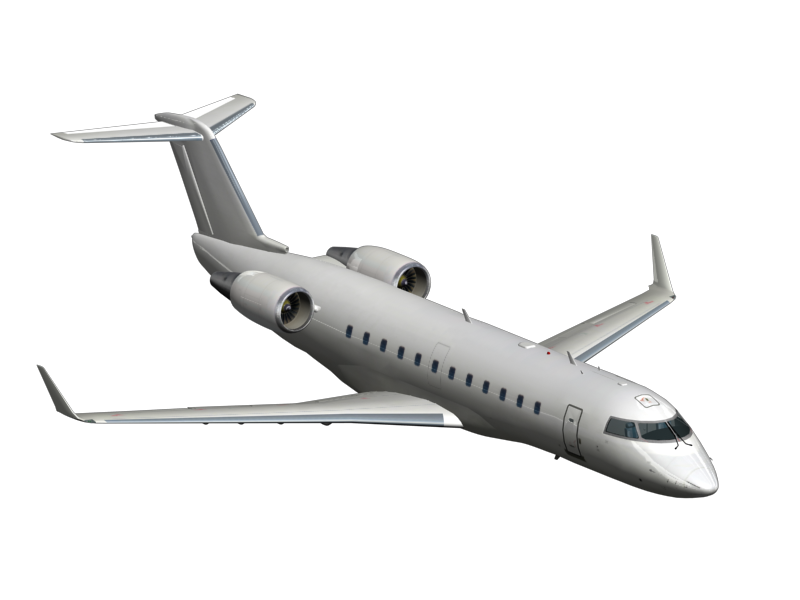
\includegraphics[width=\linewidth]{Figures/Bombardier_CRJ200}
  \end{minipage}%
  \begin{minipage}[b]{0.30\linewidth}
    \centering
    \begin{tabular}[b]{lll}
      \toprule
        \multicolumn{3}{c}{Legend} \\
      \midrule
        A & B & C \\
        0 & 0 & 0 \\
        0 & 1 & 0 \\
        1 & 0 & 0 \\
        1 & 1 & 1 \\
      \bottomrule
    \end{tabular}
    \vspace{5em}
  \end{minipage}
\caption{Figure and table side-by-side.}
\label{fig:side_by_side}
\end{figure}

\end{comment}